
\chapter{Communication System Simulation }\label{ch:simu}
In the previous chapters the components of an fiber system have been described, taking special attention to the noise that arises from the nonlinear interaction between the optical fiber and the propagating light. To obtain measurements of noise sources described in Chapter\#?\#. To detect NLPN it is necessary to have a multiple amplification segments. Thus, a long-haul fiber link is an ideal scenario given that it has more than ten fiber amplification segments where NLPN would by imprinted into the received constellation. The two other nonlinear noise sources is SPM and XPM which are present in systems with multiple channels being transmitted over the same fiber. To measure this effect a WDM scheme is also implemented to detect the interchannel interference imparted to the transmitted constellation. Both of this systems are simulated using  \emph{VPItransmissionMaker$^\text{TM}$}~\cite{transmissionvpi} also known as VPI. This software allows accurate simulations of a multitude of photonic systems including coherent optical links as a plug and play software.


With the simulated links a bit sequence will be transmitted over the system, where at the receiver side the detected constellation point will classified and decoded using different DSP schemes. The DSP algorithms that will be implemented have been discussed in Chapter\#?\#, where it is motivated when to implement and what improvement are preformed to the system. For each fiber link we will compare the proposed nonparameter nonlinear noise characterizing DSP with the DSP computed by VPI automatically. Giving us a point of reference to determine if there is an improvement in transmission length when using a more robust DSP scheme. 

 







\section{VPI Detection scheme }\label{sec:VPIdec}


Each communication link was intended to give insight about the relation ship between a physical variable or system architecture and the SER of the received signal. The components used to build this communication link have been described in Chapter \#?\# in this section some additional comments on the simulation parameters and processing scheme will be done. For all architectures the detection and modulation were preformed with he same modules in VPI, to measure the difference between using different fiber lengths, launch power and amount of channels transmitted. When the system are simulated VPI preforms a numerical simulation propagation of the transmitted symbol through the specified link. In the receiver side VPI automatically preforms some signal processing to retrieve the IQ parameters of the received symbol. This signal processing is preformed automatically by the used VPI module.      
 	



\begin{figure}[h!]
\centering
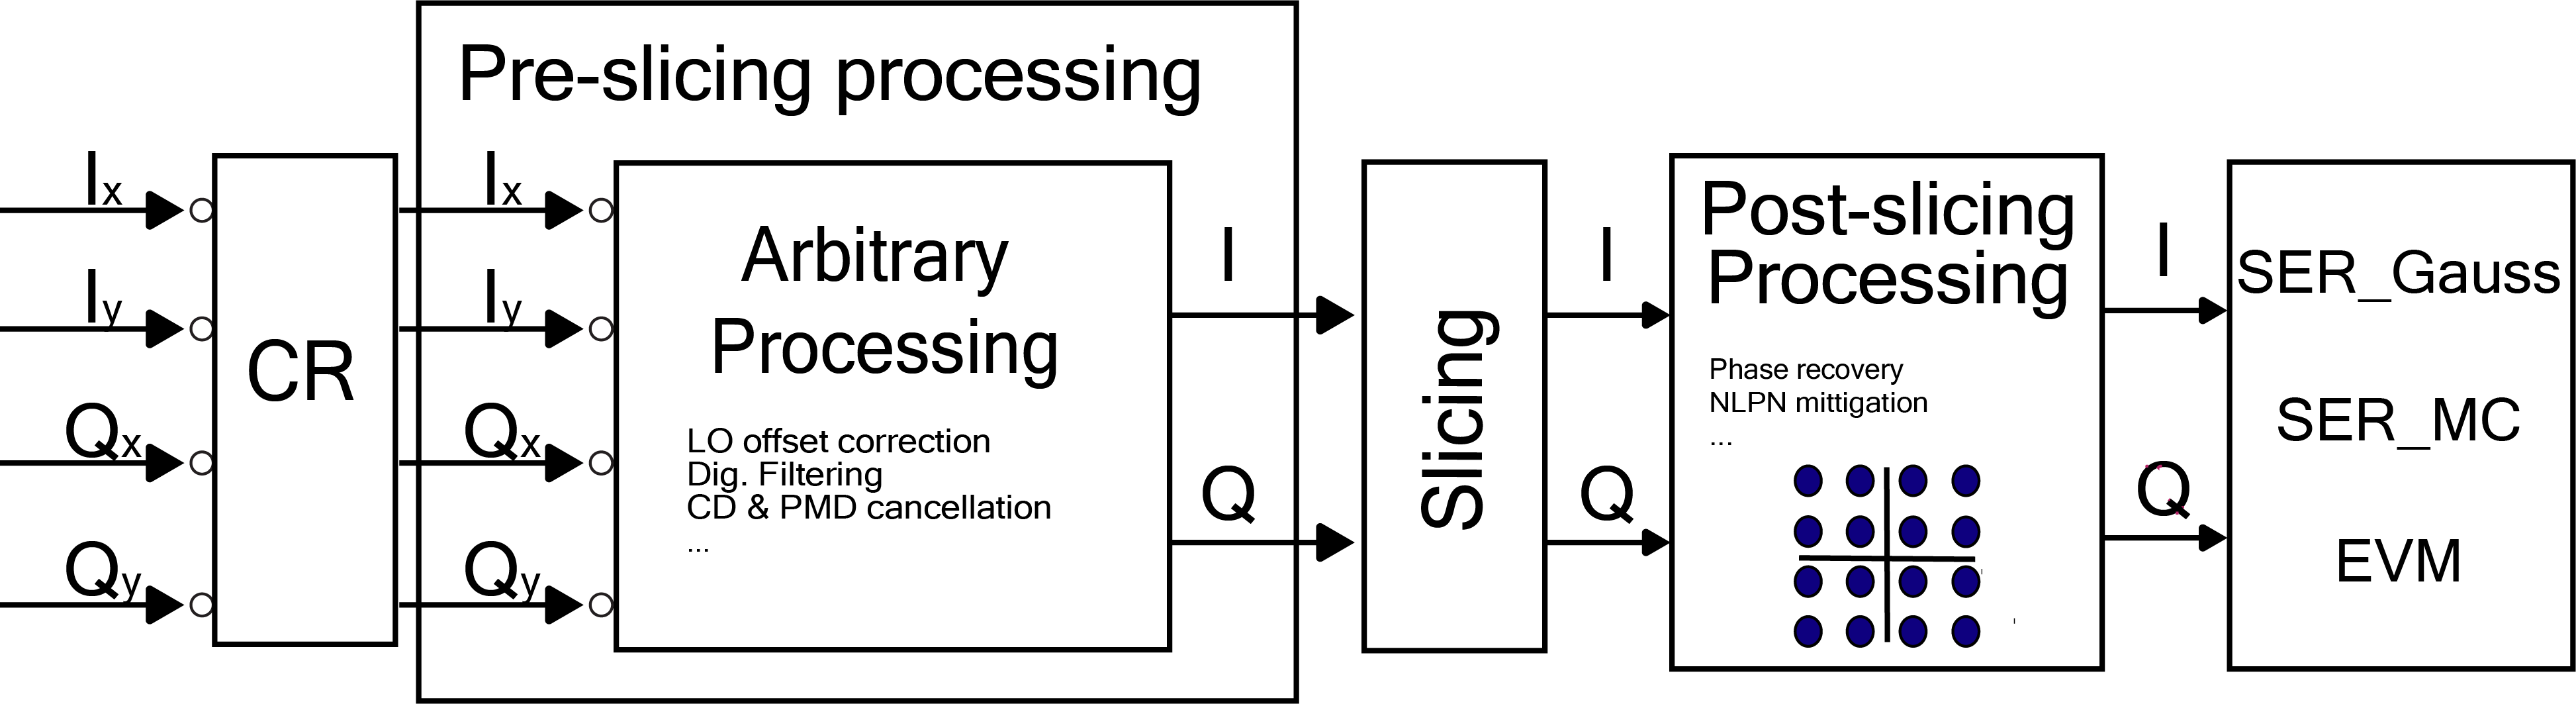
\includegraphics[width=\linewidth]{DSPscheme.png}
\caption{Block diagram of the signal processing preformed by VPI after detecting the IQ parameters of a transmitted symbol. }
\label{fig:dspvpi}
\end{figure}


Throughout all simulated communication systems, the detection processing scheme follows the same block architecture. After retrieving the IQ parameters with the detection scheme discussed in Section\#?\# the VPI module process the symbols as shown in Figure~\ref{fig:dspvpi}. Each block accepts inputs to alter its behavior as needed to preform compensation or retrieve the symbol processed. The signal processing scheme implemented by VPI receives the transmitted \emph{IQ} complex samples for orthogonal polarizations \emph{x} and \emph{y} and performs clock recovery in order to remove any possible time delays between the transmitted and received symbol sequences. Selecting one time sample to preform metric calculation is called “slicing”, which has the same meaning as “sampling“ in conventional BER estimator.  Generally, the processing scheme is divided into  Pre- and Post-Slicing DSP procedures. As is shown in the block diagram custom DSP procedures can be applied before and after slicing to correct or mitigate impairments in the signal like CD, LO offset and NLPN. If the correction algorithm is timing dependent it is preformed before slicing to have the information for each symbol. 


Retrieving the IQ components is done in post-slicing because we are not considering time dependent phenomena. With the IQ components extracted from VPI the DSP is done in python as was described in Chapter\#?\#. For each communication link the DSP implemented is used to improve the classification of the detected symbol, ultimately lowering the SER of the link. The receiver has a run time simulation of 0.128~$\mu s$ at symbol rate of 32~$Gbuad/s$ transmitting a total of $2^{12}=4096$ symbols per frame. This is the total length of the simulation carried out for each frame or transmission length of the simulation.


\section{Coherent Communication System Implementation}

High capacity, low latency and other technological advantages like transparent amplifiers and routers have made optical fiber the most implemented technology for long distance communication, and is being currently deployed in the access network as well. In this section a 32~Gbuad 16QAM transmitter was simulated in different architectures to observe the effects of NLPN, SPM and XPM. In this section we will describe each of the communication systems simulated and the data collected for different configuration will be discussed as well. 


\subsection{Gordon-Mollenauer effect \& SPM in a Long-Haul Fiber Link }
A system with a single frequency channel transmitted over lumped amplification is ultimately limited by the NLPN and SPM. To measure the effects of this nonlinear noises sources the fiber link shown in Figure~\ref{fig:1chlink} was simulated. This system can be implemented to sweep over launch power, fiber length and amount of fiber spans in the system. With this scheme we can observe the effects of NLPN and SPM on the transmitted constellation and preform DSP to optimize the decision regions to classify each symbol.


\subsubsection{Architecture}
A long-haul fiber system is composed of multiple segments of fibers spans with their corresponding amplification one after the other. To simulate a long fiber a loop block is used to propagate the signal over a  $80~km$ fiber segments as many times as desired, a set of 64 spans was simulated making the total fiber length a maximum of 5120~km. After each loop the transmitted signal can detected without altering the system. 
 

\begin{figure}[h]
\centering
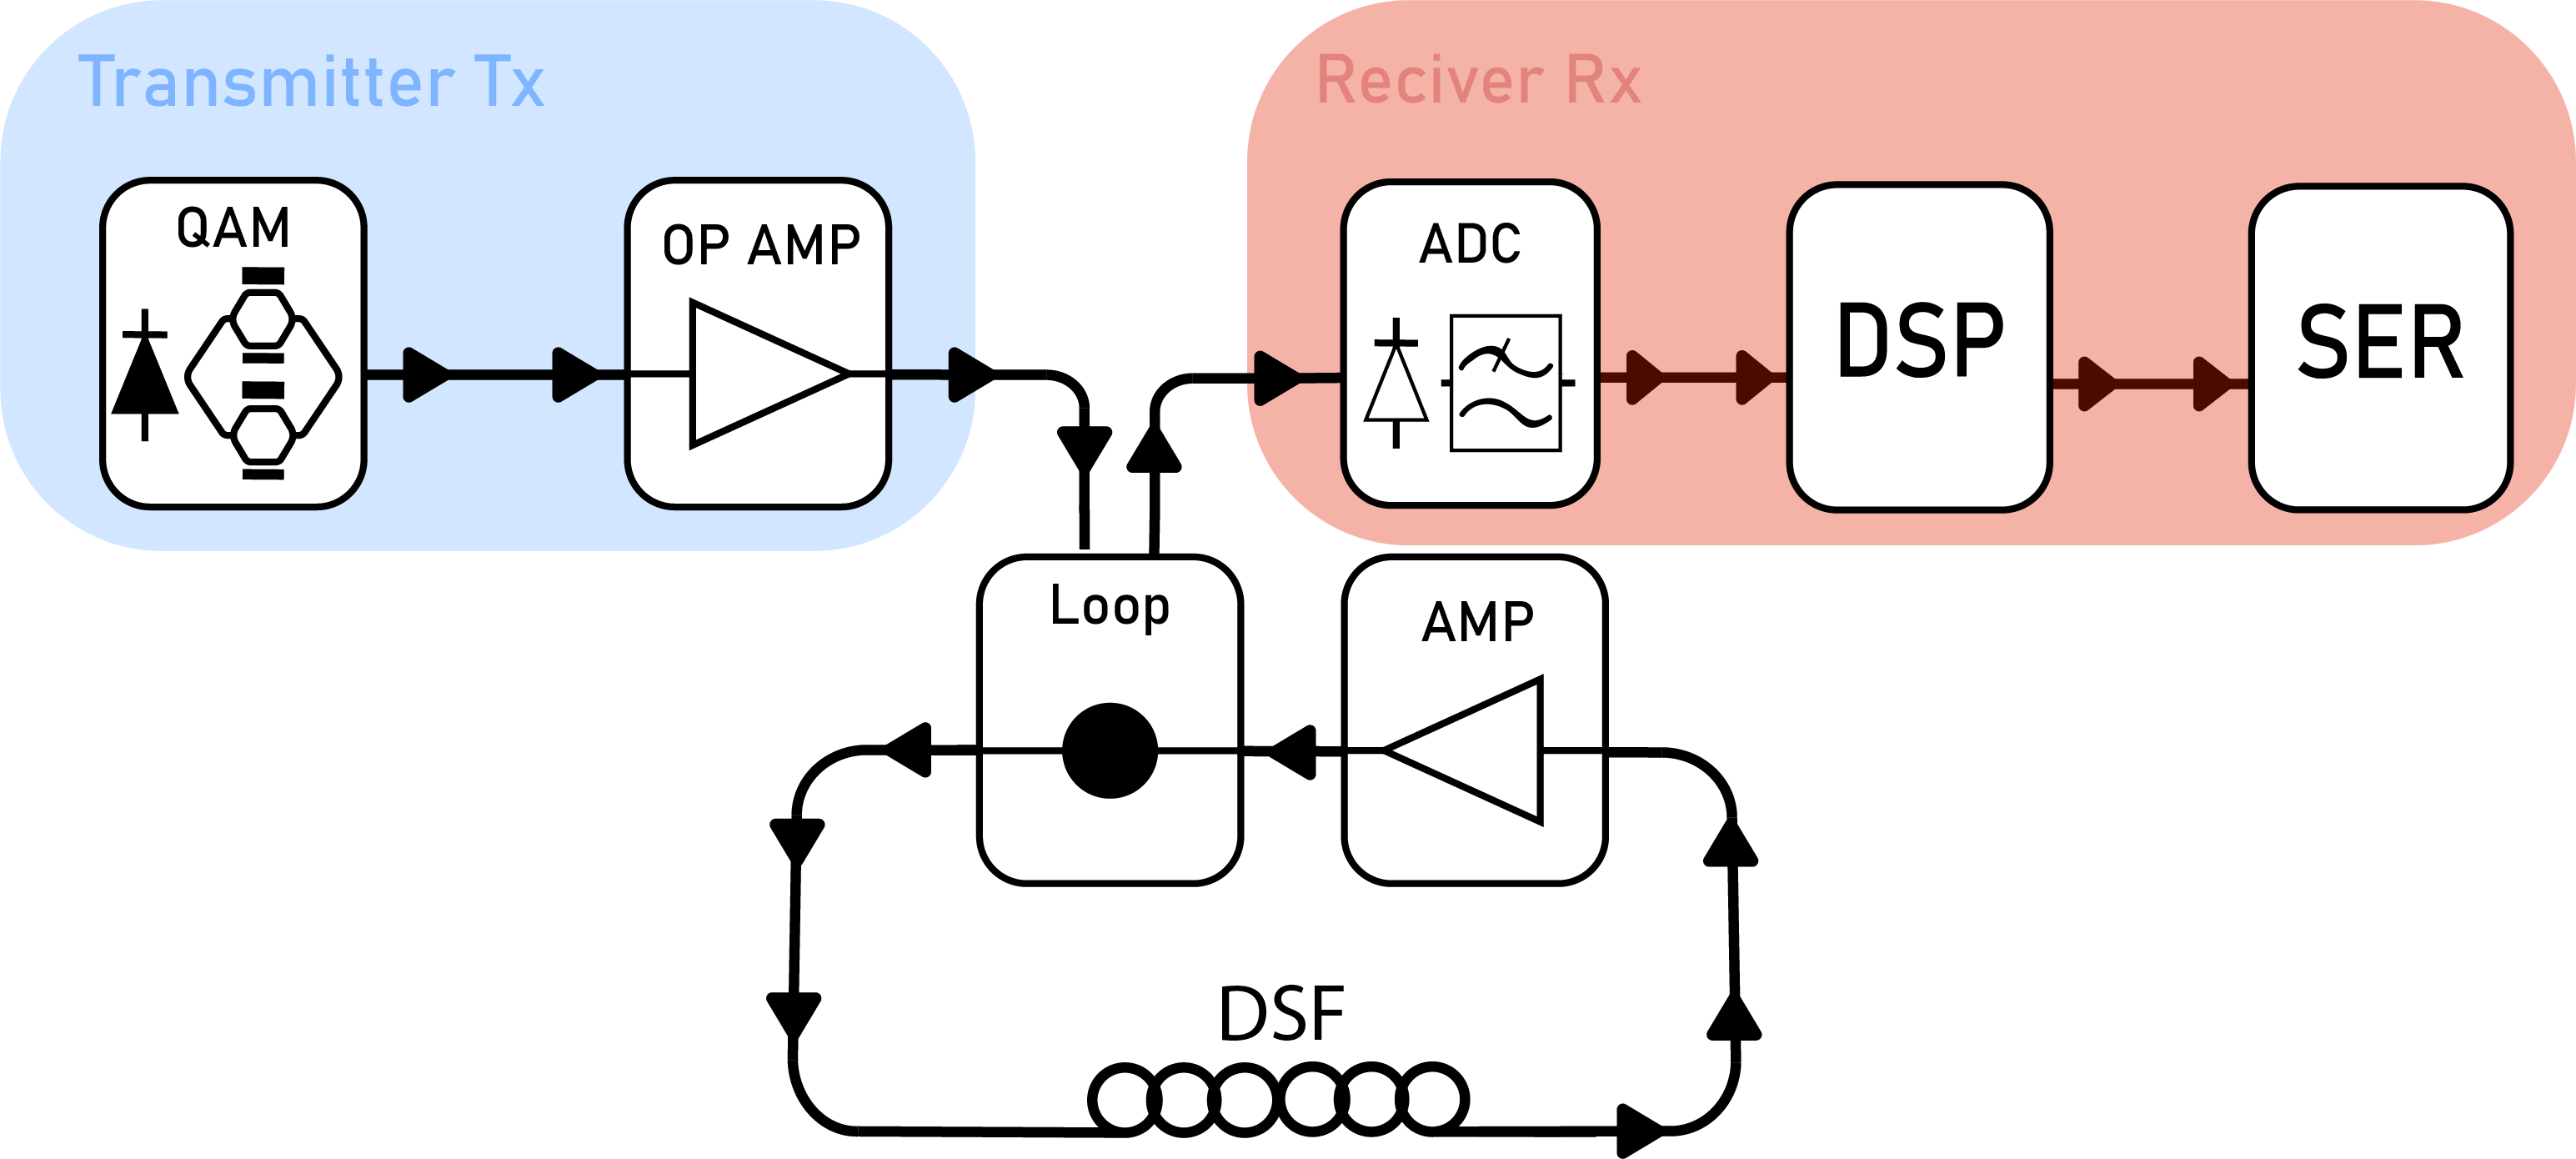
\includegraphics[width=0.7\linewidth]{DCFscheme.png}
\caption{Architecture of a single channel fiber link. The transmitter is composed of a optical carrier and modulator, that permits independently setting the launch power. The propagating fiber implemented is a DSF with inline amplification to compensate for fiber losses, the amplifiers simulated add small amounts of AWGN to isolate the effects of NLIN. At the receiver side a ADC retrieves the digital IQ parameters and send them to the DSP which improves the single quality that is quantified by the SER. }
\label{fig:1chlink}
\end{figure}
  
Nonlinear effects are prevalent in this system due to the fibers relatively large length and nonlinear coefficient. With this system we intend to get a understanding on the effects of applying DSP on the received signal. It would be advantageous if we could preform some digital processing and improve the quality of the signal. Resulting in a system that can be transmitted a longer distance or has a more reliable connection. The detected signal is imprinted with a phase rotation from NLPN and SPM, however SPM is very weak compered to NLPN so we will focus primarily in this source of noise. As a reference for 30 spans of DSF fiber  upper bound channel power (as discussed in Section \#?\#) $P_{ch}\le0.4~mW$  acquires a phase shift $\phi_{SPM}< 1.3$~mrad, compared to a a NLPN phase shit of $\phi_{NLPN}< 92.6$~mrad. Thus, for this simulation even though SPM is present it is not the dominant noise source in the system.  


  
\subsubsection{Transmission Measurement for a Single Channel 128~Gbit/s  System}

As was discussed in Section\#?\# nonlinear effects depend on the fibers length, the amount of fiber segments and the transmission power. A fixed fiber length of $80~km$ has been chosen for convenience, thus determining the optimal launch power is necessary. An optimal lunch power would be such that it presents high enough OSNR for re-transmission, ultimately increasing the systems reach by improving the signal quality. To decode a HOM format it is necessary to have a clear signal with a high OSNR, this can be achieved by operating at high launch powers. However, if the launch power is to intense the OSNR will decreased do to the nonlinear noise added to the signal. Balancing this trade off is important for the system, given that at the proper operating power a more reliable and further reaching system can be achieved. A power sweep was preformed to determine the optimal power and observe the effect on the transmission distance and DSP schemes.

\begin{figure}[h]
  \centering
   \subfloat[]{\label{fig:017mw}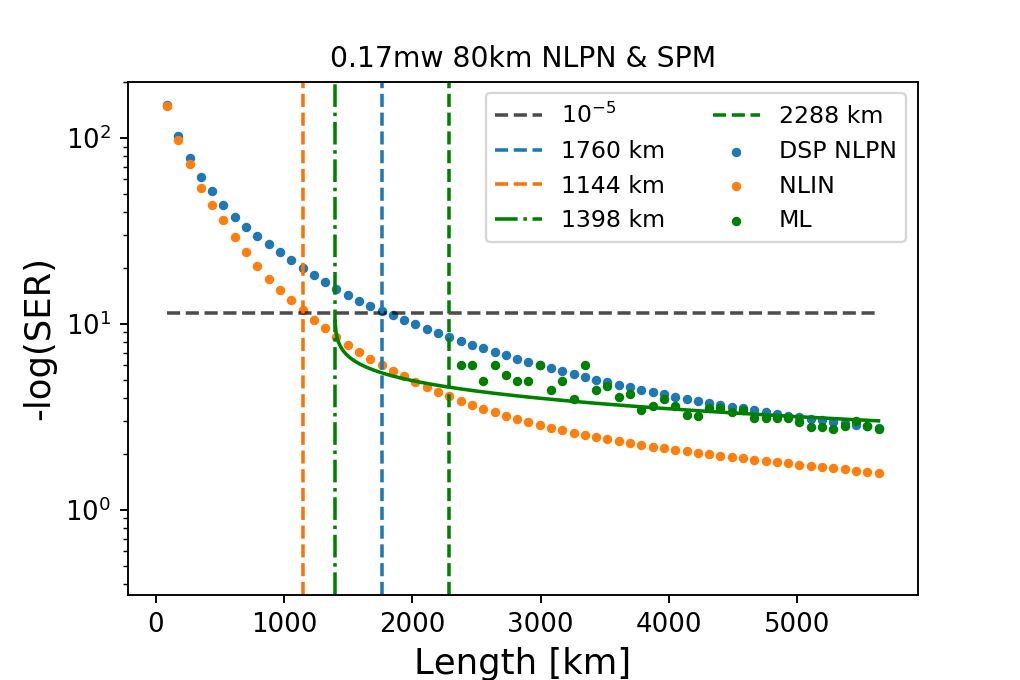
\includegraphics[width=.45\textwidth]{SERlogmlDSF017mw80l64n.png}}
  \qquad
  \subfloat[]{\label{fig:025mw}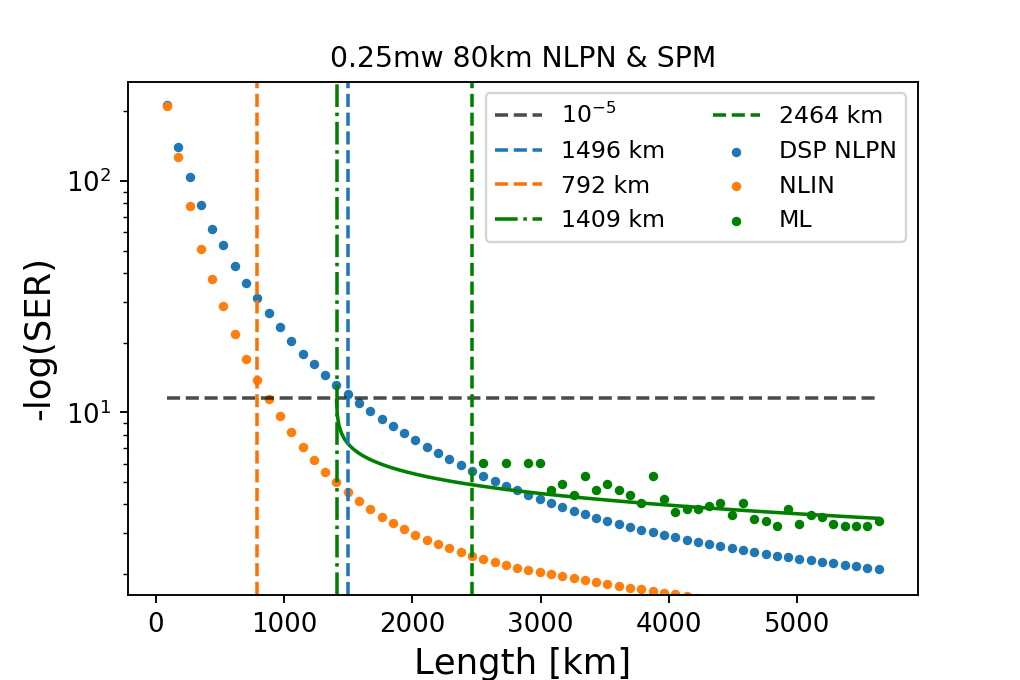
\includegraphics[width=.45\textwidth]{SERlogmlDSF025mw80l64n.png}}
     \qquad
    \subfloat[]{\label{fig:05mw}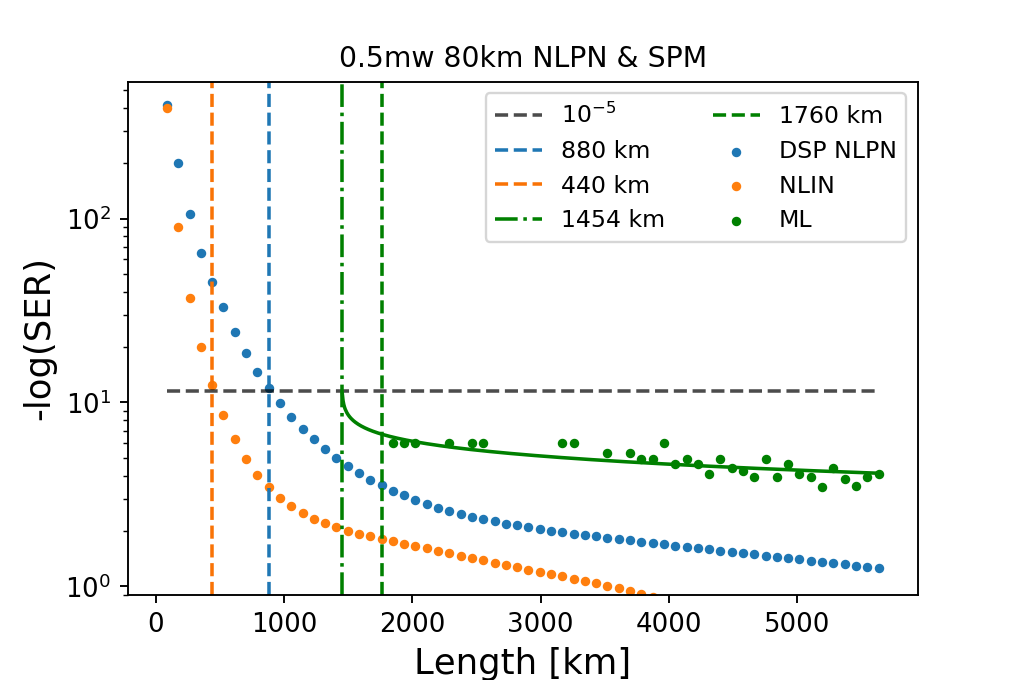
\includegraphics[width=.45\textwidth]{SERlogmlDSF05mw80l64n.png}}
    \caption{Single Channel 16QAM long-haul link operating at a low launch power. At this operating power the system present a small amount of nonlinear noise, making AWGN the main limitation.  }
    \label{fig:lowP}
\end{figure}
 
To determine the effect of nonlinear noise on the system a low launch power were first investigated. Even thought the launch power is relatively low $P_{ch}\le 0.5$~mW the $OSNR\ge 25 $dB can be reliably detected because in this simulation we isolate the NLIN by simulating low noise figure amplifiers adding a small amount AWGN. A \textit{reliable detection} is amused to be a system that has a SER$>10^{-5}$, which is the same as a communication link that preforms one mistake every hundred thousand symbols. The phase shift acquired in this datasets is $\phi_{SPM}\le 3.8$~mrad and $\phi_{NLPN}\le 115.8$~mrad, making it a good region to detect primarily NLPN. 


 From the simulation we can retrieve the IQ parameters  with all the NLIN acquired from transmission, represented by the color orange in all the plots in this chapter. From this dataset all DSP scheme are computed, represented in this section by the color blue for the analytically derived scheme and green for the nonparamter ML algorithm proposed in this report. The horizontal bars in all plots in this chapter represent the fiber span at which the system (orange) or the DSP schemes (blue, green) stopped being reliable. The dashed horizontal bar for the ML implementation is directly computed NLIN dataset, while the dashed-dotted line is determined by an exponential function fitted to the computed ML data set. This fitting is preformed due to a abrupt change in the green scattered points, in the next section this effect will be further discussed. This fitting determines an approximate maximum reliable transmission distance if the change in the SER predicted by the ML algorithm had an exponential change. However, the change in this ML SER function is much faster than a exponential fitting. Meaning that the maximum reliable transmission distance could fall in between the two green horizontal lines, this region will be refereed to as the \textit{optimal prediction region}  (OPR). 
 
 From Figure~\ref{fig:lowP} we can determine that there seems to be a tendency for the ML algorithm to preform better for higher launch power. This is determined by the shift to longer transmission length of the green horizontal bars. We can notice that at a operating power of $0.5$~mW (Figure~\ref{fig:017mw}) the OPR at a minimum of 1454~km  starts to out preform the analytical DSP scheme. 
\begin{figure}[h]
  \centering
  \subfloat[]{\label{fig:15mw}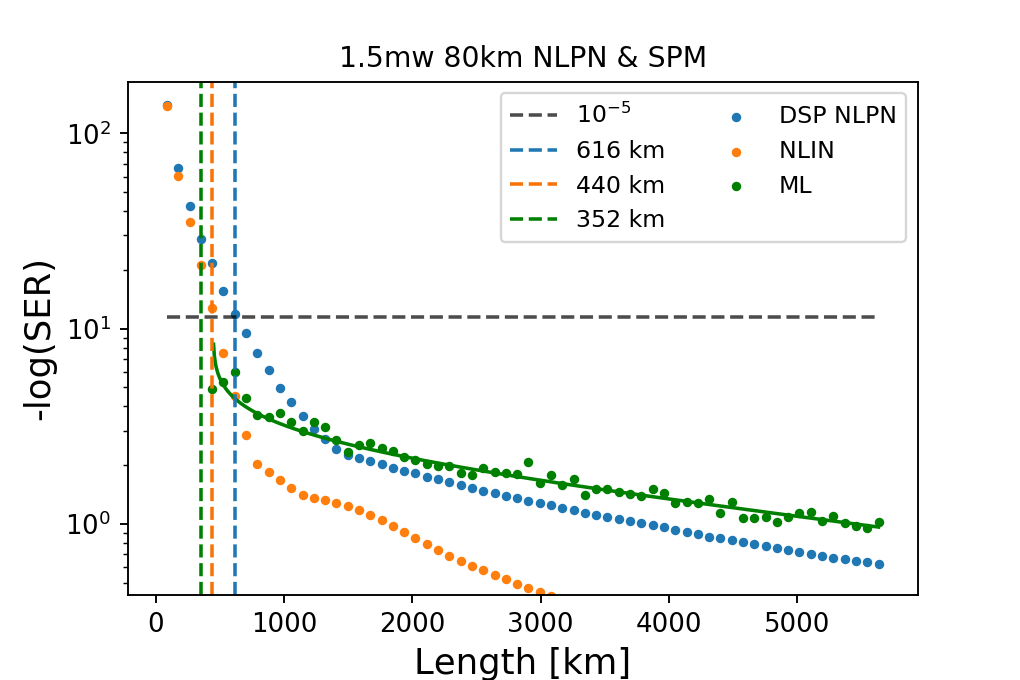
\includegraphics[width=.45\textwidth]{SERlogmlDSF15mw80l64n.png}} 
\qquad
\subfloat[]{\label{fig:2mw}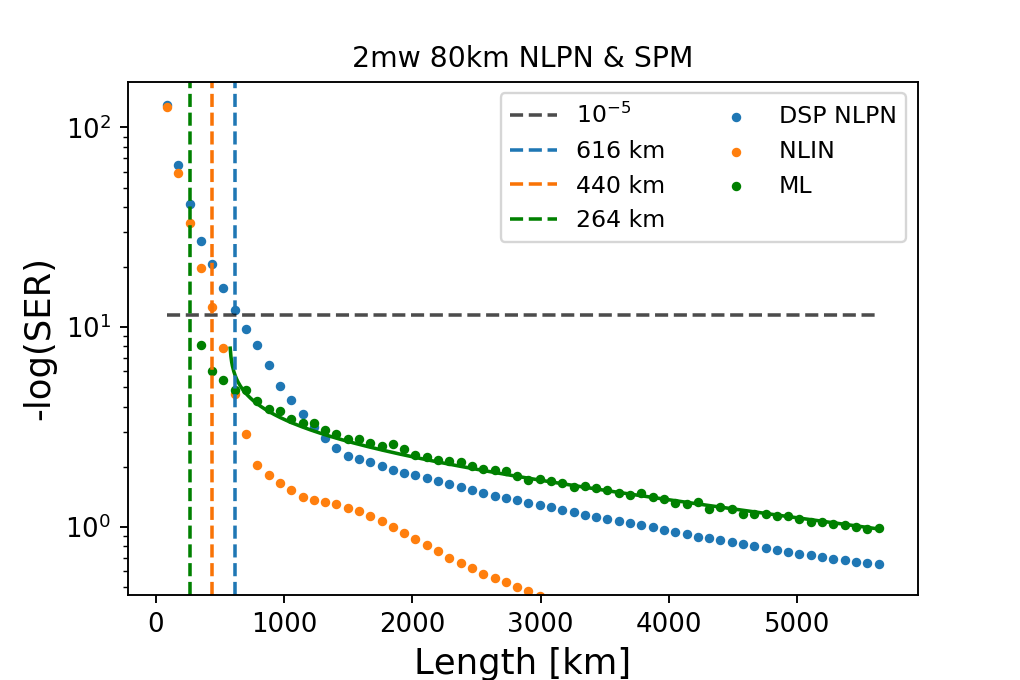
\includegraphics[width=.45\textwidth]{SERlogmlDSF2mw80l64n.png}}       
  \caption{Single Channel 16QAM long-haul link operating at a high launch power. At this operating power the system present a large amount of NLIN critically reducing the performance of the system. }                                                                                                                                                                                                                                                                                                                                                                                                                                                                                                                                                                                                                                                                                                                                                                                                                                                                                                                                                                                                                                                                                                                                                                                                                                                                                                                                                                                                                                                                                                                                                                                                                                                                                                                                                                                                                                                                                                                                                                                                                                                                                                                                                                                                                                                                                                                                                                                                                                                                                                                                                                                                                                                                                                                                                                                                                                                                                                                                                                                                                                                                                                                                                                                                                                                                                                                                                                                                                                                                         
 \label{fig:highP}
\end{figure}
Given this observation it could be consider that ranking up the launch power would produce a further reaching system. However, it can be seen in Figure~\ref{fig:highP} that all DSP scheme quickly start to fail with the increase in NLIN. For 2~mW launch power after 560~km of fiber the signal would have acquired a phase shift $\phi_{SPM}\le 15.4$~mrad and $\phi_{NLPN}\le 108.1$~mrad, even thoguht this might seem like is a small phase shift the signal is mixed much faster than for lower powers making this acquired phase shift corrupt the signal faster.
Through the power sweep it was determined that the optimal launch power was 1~mW (Figure~\ref{fig:1mW}) due to the overall shift to longer distance in the OPR of the system. The acquired NLIN phase shift at 2288~km is $\phi_{SPM}\le 7.7$~mrad and $\phi_{NLPN}\le 200.7$~mrad. Notice that even thought the acquired phase shift is large than the one computed for a 2~mW the performance of the system is better. In Figure~\ref{fig:1mWOSNR} the OSNR for each fiber span is shown, the OSNR was extracted from the simulation which computes the \textit{error vector measurement} directly from the desired constellation giving off a smooth functions.
  
  
  
  
\begin{figure}[h]
\centering
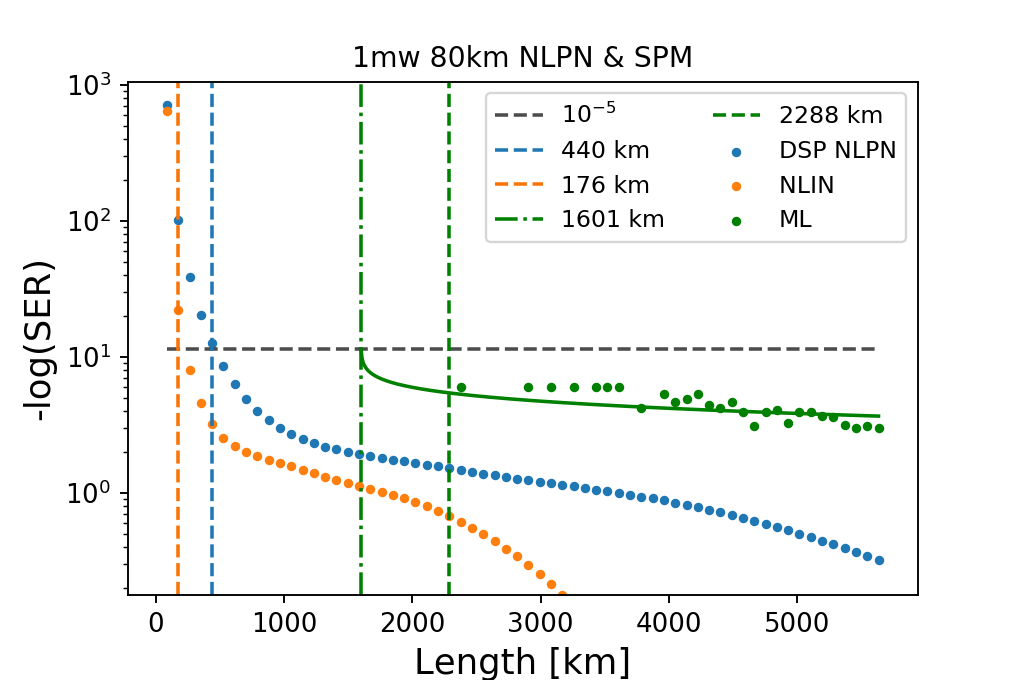
\includegraphics[width=.7\textwidth]{SERlogmlDSF1mw80l64n.png}
\caption{Single Channel 16QAM long-haul link operating at the optimal launch power of 1~mW. At this operating power the system present the optimal balance between optical power and induce NLIN phase shift. The signal preserves its information allowing it to be accurately decoded at further distances even thought it has acquired a maximum phase shift $\phi_{nl}\le 239.6$~mrad at a fiber length of 2400~km. }
\label{fig:1mW}
\end{figure}



\subsubsection{Measurement Discussion}

A few remarks should be made about the measured launch powers and their resulting SER. The lowest launch power simulated was 0.17~mW (Figure~\ref{fig:017mw}), for this system the NLPN is approximately 30 times larger than the SPM noise. Given that this system presents mainly NLPN the analytically derived DSP scheme can compensate most of this noise. With this in mind we intend to compare the performance of the ML scheme represented by the green scattered dots. For long transmission lengths it can be observed in Figure~\ref{fig:017mw} that the ML scheme tends to preform as well as the analytical DSP scheme. Suggesting that the ML scheme can effectively decrease the SER of the system but it cant outperform the prefect compensation achieve by the analytical DSP scheme. 
 In all plots the ML scheme (green scattered dots) abruptly starts making mistakes after a certain fiber length. This abrupt change from the SER is due to a limitation of the simulation preformed. A total of 4096~symbols are being simulated per frame, if one mistake is made in a dataset the SER=$24\cdot10^{-5}$ automatically failing the reliable detection condition. However, this only means that the fewer mistakes are made the more samples are needed as is known from the \textit{Law of large numbers}. Simulating for longer times could be a solution to this limitation but it is not practical for the scope of this report, given that increasing the simulation time would increase the computation time for all the project beyond what is available at my disposal.  
Due to this limitation of the simulation a exponential function was fitted to the SER predicted by the ML algorithm, represented by the solid green plot. 

For the simulation preformed the maximum transmission length would lay the region between the zero SER predicted ML algorithm (horizontal green dashed line), and the length at which the fitted exponential function (horizontal green dash-dotted line) intersects the optimal prediction boundary. The from power sweep it was determined that the optimal launch power was 1mW as seen in Figure~\ref{fig:1mW}, due to the shift of the OPR to longer transmission lengths it cen be determined that in the very list the ML processing scheme is preforming as well  as the analytical DSP. Preforming as well or better than the analytical DSP scheme is am interesting result because it suggest that a DSP scheme with no information about the system can resolve NLIN comparable to a scheme that has all the information about the links architecture.
Increasing the launch power results in critically hindering the communication link, ultimately corrupting the prediction of all the DSP schemes and reducing the transmission length. In Figure~\ref{fig:highP} it can be observed that all horizontal bars or optimal prediction lengths quickly recline to lower transmission lengths. The main take away from this simulation is that the proposed ML scheme at the optimal launch power could increase the transmission length any where from 2.5 times (same performance as the analytical DSP) to 9.4 time longer (length predicted by exponential fit), which could motivate a further investigation in this area.




\subsection{SPM \& XPM in a WDM system}

Increasing the transmission capacity can be achieved by adding more channels to the system, either by \textit{polarization division multiplexing} or \textit{wavelength division multiplexing}. In this system both of this techniques are implemented to increase the transmission capacity and explore interchannel noise. Every transmitter has two orthogonal polarization channels, a total of five transmitters in the system are used giving a 1.28~Tbit/s link. This system can be used to measure the effect of SPM and XPM, because transmitting multiple channels over a single fiber naturally increase the optical power perceived in the fiber inducing nonlinear noise. 

The fiber system implemented  induces dispersion at different rates for each communication channels. Transmission is done over NZ-DSF and the dispersion acquired is mitigated for all channels with a SC-DCF fiber. This fiber arrangement presents in total a higher nonlinear coefficient and a smaller effective areas, enhancing nonlinear noise. The high power given of by all channels together hinders the transmission length that can be achieved by increasing the NLIN present in the system.

\subsubsection{Architecture}

An advantage of the modules used in VPI are their flexibility to implement a dual polarization transmitter and  alter the operating frequency. The channel spacing between optical carriers was $50~GHz$ making this system a \textit{dense wavelength division multiplexing} architecture. The propagating fiber implemented was a 80~km NZ-DSF that induces dispersive effect on all channels of the system. Dispersion compensation is done with a 7.14~km SC-DCF that can preform an close to an ideal compensation. The maximum transmission length was 10 spans of 87~km fiber, equal to 870~km. It was assumed that all fibers were polarization mode preserving for simplicity . The fiber loss amplification preformed is done with a amplifies with a low noise figure, such that the dominant source of noise is the NLIN source that are present in the WDM system.  

    
\begin{figure}[H]
\centering
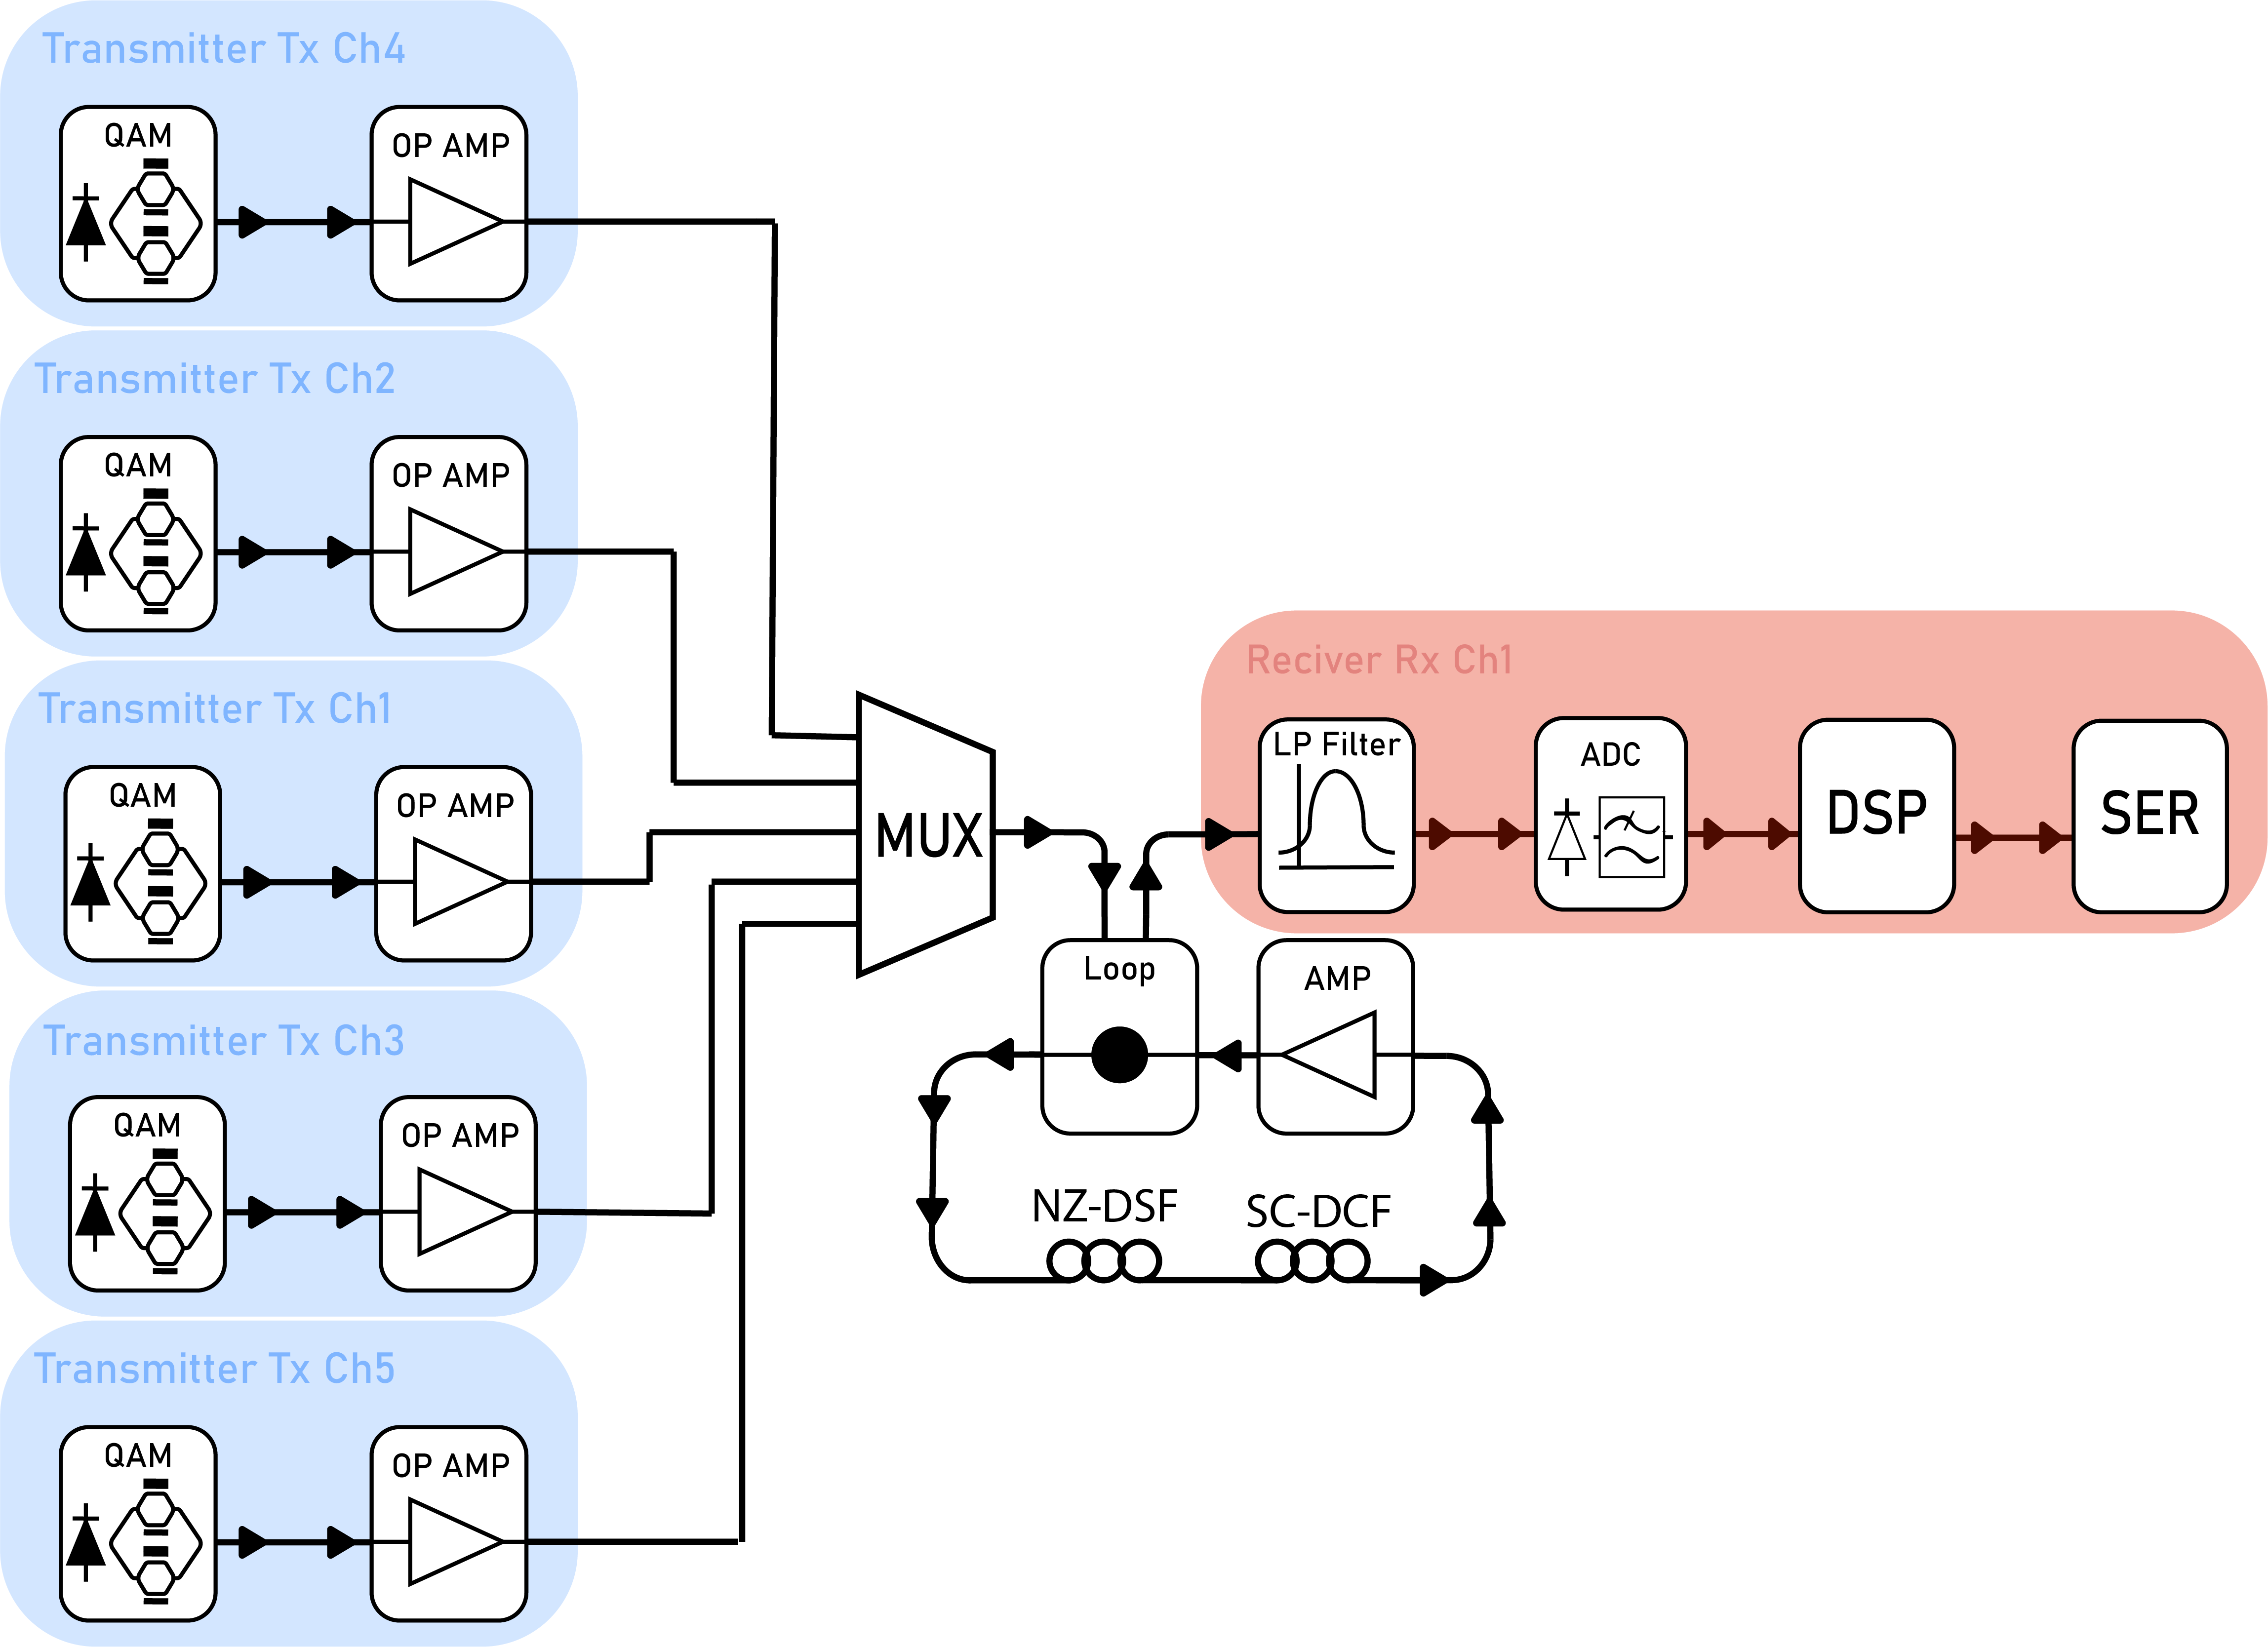
\includegraphics[width=0.6\linewidth]{WDMscheme.png}
\caption{Architecture of 5 channel WDM dual polarization fiber link. The transmitter is composed of a dual polarization optical carrier  and modulator. The launch power can be independently adjusted as desired. The fiber segment used produce a total signal that present a small amount of dispersion than dose not critically hinder the system. At the receiver side a ADC retrieves the digital IQ parameters and send them to the DSP that tries to improve the SER. }
\end{figure}

All block used for the simulation in VPI are the same as in the previous link. Thus once again the amplification preformed for each fiber segment is almost ideal, adding a small amount of AWGN to the signal. This is done to isolate the NLIN that is in the system and focus on the nonlinear effects present in the link. In this system XPM noise is present for any system that has a channel power $P_{ch}>0.07mW$ which would be any relatively realistic implementation. 


\subsubsection{Transmission Measurement for a $5\times 256 Gbit/s $}
 The measurements preformed were done in the same manner as for the previous long-haul communication channel. To find the optimal launch power a sweep was preformed and the SER was measured. In Figure~\ref{fig:powWDM} the SER for the signal with all the NLIN is represented by the blue scattered points. Once again the ML scheme suggest is represent by the green scatter points, with its corresponding exponential fit as the green solid function. 
 
\begin{figure}[h]
\centering
\subfloat[]{\label{fig:wdm025}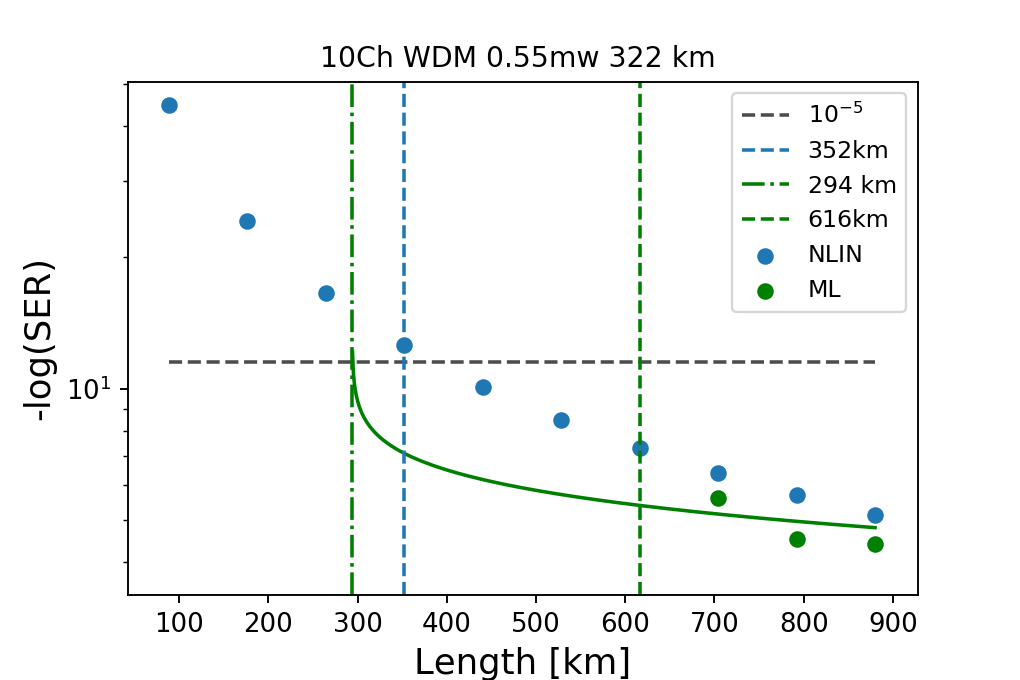
\includegraphics[width=.45\textwidth]{SERlogmlWDM-6dBmw.png}}
\qquad
\subfloat[]{\label{fig:wdm063}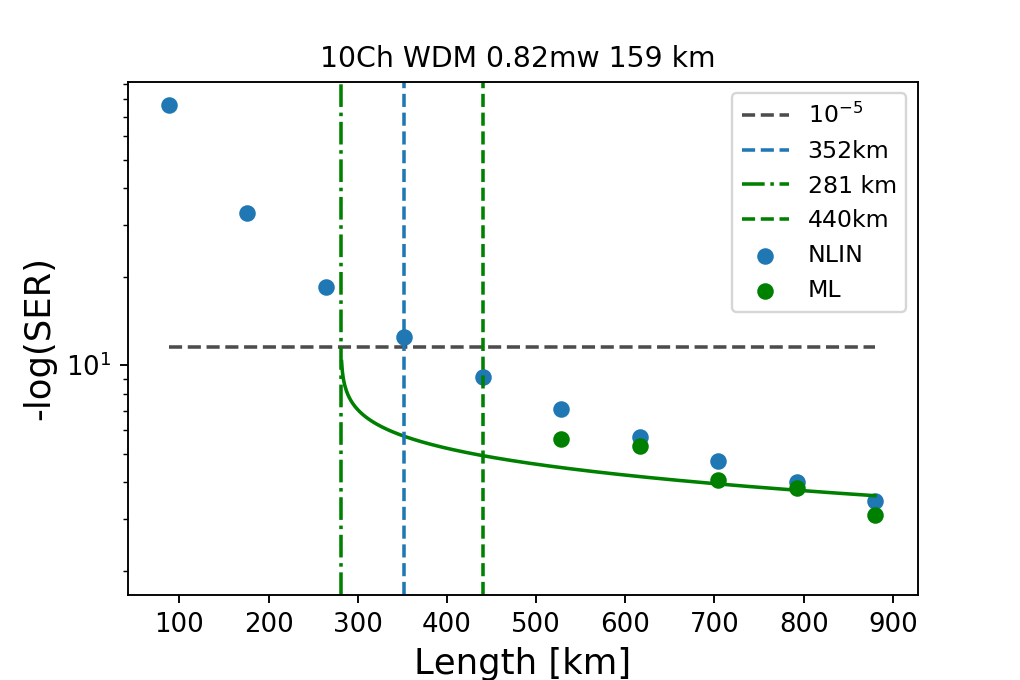
\includegraphics[width=.45\textwidth]{SERlogmlWDM-2dBmw.png}}
\qquad
\subfloat[]{\label{fig:wdm079}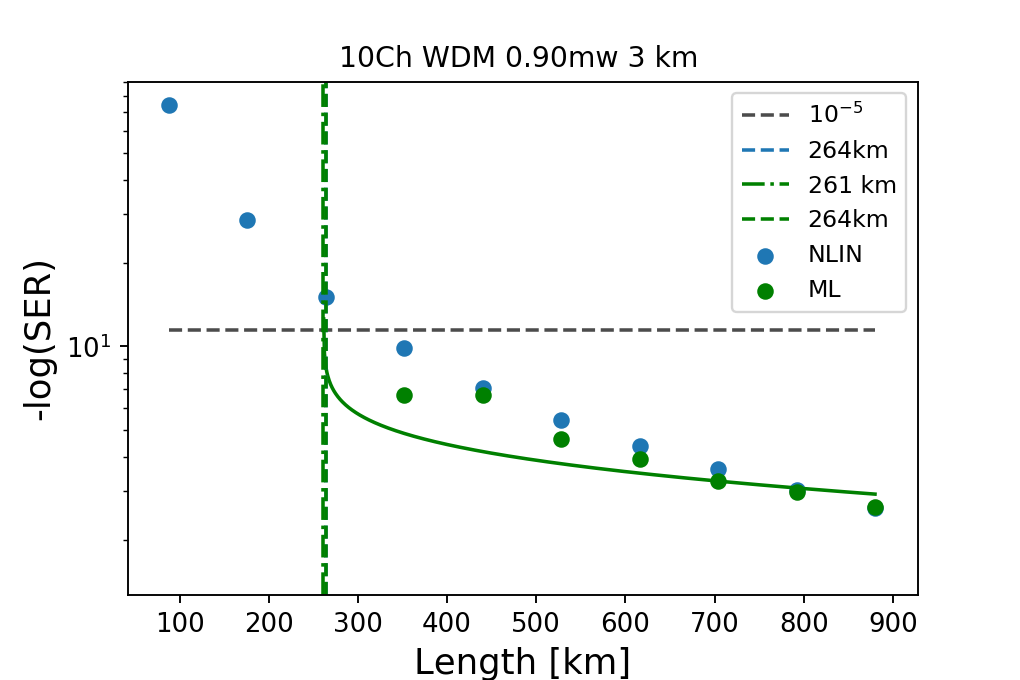
\includegraphics[width=.45\textwidth]{SERlogmlWDM-1dBmw.png}}
\qquad
\subfloat[]{\label{fig:wdm1}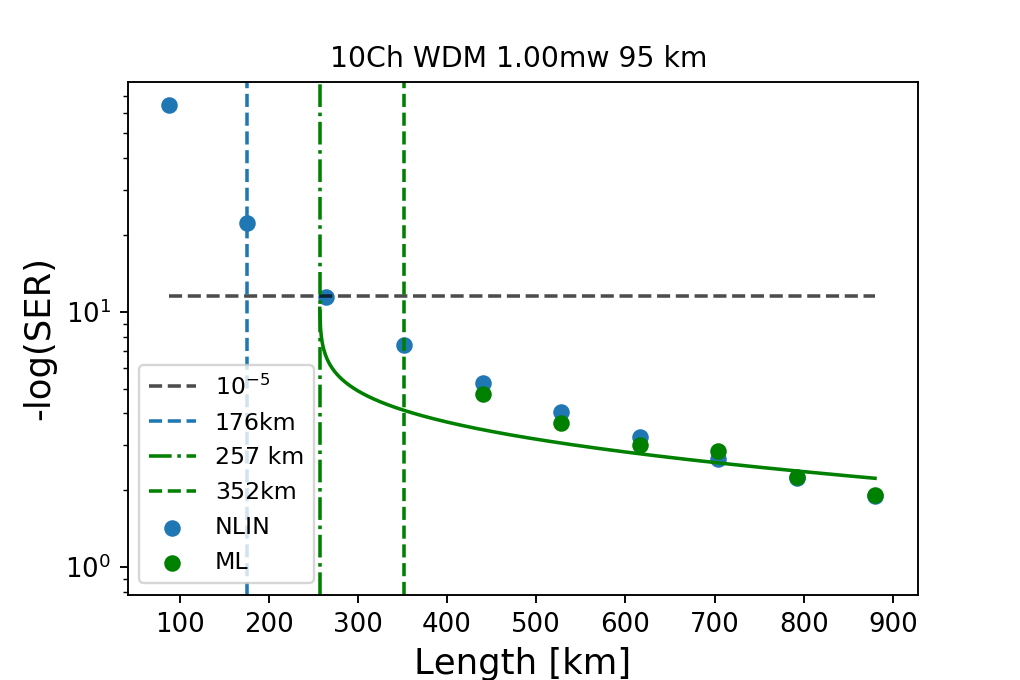
\includegraphics[width=.45\textwidth]{SERlogmlWDM0dBmw.png}}
\caption{Ten channel WDM system power sweep measurements. For this system architecture it can not be determined if the ML algorithm has any effect on the systems performance. In general the ML DSP scheme has a comparable transmission length as the detection scheme implemented by VPI.  }
\label{fig:powWDM}
\end{figure}

From the WDM simulation preformed it can not be determined if there is a benefit on implementing ML. This result can suggest that XPM is a time dynamic effect which can not be resolved with the DSP that is being preformed.


\subsubsection{Measurement Discussion}

Extending the transmission length using ML was the overall objective for this simulation. However, the data suggest that a considerable difference can not be achieved with the DSP scheme implemented. In Figures~\ref{fig:wdm025} a low launch power is tested and it can be determined that some improvement is achieve by the ML scheme, given that the OPR extends further than the optimal transmission length determined by VPI for the signal with all the NLIN. But since the optimal transmission length determined by VPI lays inside the OPR it is not clear if there is a benefit to implementing ML.

When the launch power is further increased Figure~\ref{fig:wdm079}-\ref{fig:wdm1} it seems like there is a improvement in implementing ML over VPI. The limitation is that the transmission length is shorter than for previous launch powers, making it an sub optimal operating power. What this results suggest is that XPM is a noise source dynamic in time and can not be compensated for in post-slicing processing as mentioned in Section~\ref{sec:VPIdec}. What can be said about this simulation is that XPM can not be compensated with this ML DSP scheme, but it could be used with other technologies to improve the general reliability of the system. 